%% =================================================================
%% main.tex -- Science Advances v0 draft
%% Title: Decoding subjective object-based attention from EEG in
%%        naturalistic multi-object scenes via cross-attention fusion.
%% Project: EEG_Viz_Att   |   Author: jc (paulxusilk@icloud.com)
%% Draft date: 2026-05-20 | Subjects: N=2 pilot (zfn-0507, zxc-0516)
%% =================================================================
\documentclass[12pt]{article}

% Science-recommended style (do NOT add external packages).
\usepackage{sty/scicite}
\usepackage{times}
\usepackage[]{url}
\usepackage{graphicx}
\graphicspath{{figures/}}

% Page setup per scifile.tex.
\topmargin 0.0cm
\oddsidemargin 0.2cm
\textwidth 16cm
\textheight 21cm
\footskip 1.0cm

\newenvironment{sciabstract}{\begin{quote} \bf}{\end{quote}}
\renewcommand\refname{References and Notes}

\newcounter{lastnote}
\newenvironment{scilastnote}{%
\setcounter{lastnote}{\value{enumiv}}%
\addtocounter{lastnote}{+1}%
\begin{list}{\arabic{lastnote}.}{\setlength{\leftmargin}{.22in}}{\setlength{\labelsep}{.5em}}}{\end{list}}

\title{Decoding subjective object-based attention from EEG in
naturalistic multi-object scenes via cross-attention fusion of
neural and visual representations}

\author
{Authors blinded for review$^{1\ast}$\\
\\
\normalsize{$^{1}$Affiliation withheld}\\
\\
\normalsize{$^\ast$Correspondence: paulxusilk@icloud.com}
}

\date{}

\begin{document}
\baselineskip24pt
\maketitle

% --------------------------------------------------------------
% ABSTRACT  (~ 125 words; Science Advances has no hard limit but
% recommends an unstructured one-paragraph abstract.)
% --------------------------------------------------------------
\begin{sciabstract}
Modern brain decoders can reconstruct what was \textit{shown} to the
visual system, but they cannot dissociate the stimulus from what the
brain chose to \textit{attend to}. We collected an EEG--gaze
dataset (40 LVIS-on-COCO categories, 6376 epochs per subject in two
pilot subjects) in which each natural multi-object image is shown
multiple times under different non-spatial semantic attention HINTs,
and we built a cross-attention transformer that fuses scalp EEG
with frozen vision-transformer image embeddings to predict the
attended category. The fused model reaches top-1
$\approx 30\%$ and top-5 $\approx 68\%$ on a 40-way task while a
matched image-only baseline reaches only $\approx 23\%$ and
$\approx 64\%$, demonstrating that EEG contributes attention-specific
information beyond visual priors. Single-image hint-swap contrasts,
overlap-corrected ERP analysis, and within-image LDA decoding
together rule out trivial image-, position-, and stimulus-rate
confounds. The dataset and benchmark establish a state-driven (rather
than stimulus-driven) decoding regime.
\end{sciabstract}

% --------------------------------------------------------------
% INTRODUCTION
% --------------------------------------------------------------
\section*{Introduction}

Recent advances in EEG image decoding can reconstruct images and
identify object categories from scalp EEG with surprising fidelity
\textit{(1--3)}. These systems answer a single question: ``what was
\textit{shown} to the brain?'' They do not, however, address the
complementary question of what the brain \textit{chose to attend to}
when the eyes received the same retinal input.  This distinction is
central to vision: under fixed gaze, selective covert attention
modulates neural responses across early visual and parietal cortex,
yet stimulus-driven decoders are agnostic to those modulations
\textit{(4--6)}.

A handful of EEG selective-attention studies have begun to bridge
this gap (Yao \textit{et al.} 2025 \textit{(7)}, who decoded which of
two superimposed videos a subject attended to). They remain limited
to two-way tracking and synthetic mixtures, leaving open whether
EEG carries enough information to read attention out at the
\textit{object} level in naturalistic multi-object scenes.

We approach the problem from a deliberately different angle.  Rather
than constructing artificially overlaid stimuli, we present full
natural photographs containing $K=2$ to $4$ recognizable target
objects from a 40-class LVIS subset \textit{(8,9)}, and we present
each image multiple times across the experiment under different
\textit{HINT} cues that designate which target the subject must
covertly attend to.  Within an image, all low-level statistics --
luminance, contrast, object positions, spatial frequencies -- are
identical across HINT conditions; the only thing that changes is the
attended object.  This design isolates state-driven from
stimulus-driven neural variance by construction (Fig.\,1, top), and
it makes possible a fully linear ``hint-swap'' contrast: same image,
two HINTs, the difference must be attention.

We then ask a deep-learning question: can a model that fuses EEG with
a frozen image representation predict the attended category beyond
the level achievable by image features alone?  If yes, the EEG
stream carries genuine attention information that is independent of
the image; if no, image priors dominate and the EEG is decorative.
We answer this question affirmatively with a cross-attention
transformer that fuses an ATM-style \textit{(1)} EEG encoder with a
frozen ViT-B/32 \textit{(10,11)} image encoder.  Across two pilot
subjects, the fusion model achieves a top-1 accuracy of
$30.7\%$ and $29.6\%$ (zfn-0507 and zxc-0516 respectively) on a
40-way task -- $+7.7$ and $+9.1$ percentage points above the
image-only baseline and $+25.7$ and $+25.3$ pp above the EEG-only
baseline.

Our contributions are: (i) a within-image attention-modulation
dataset and paradigm built on naturalistic LVIS-on-COCO scenes that
is fully open and re-usable; (ii) an overlap-correction methodology
(rERP deconvolution) that recovers single-event ERPs from a short
rapid-serial-presentation stream; (iii) a benchmark of three
baselines and a cross-attention fusion model with explicit
within-image controls; and (iv) a set of diagnostics --
within-image decoding, signed-permutation hint-swap, and
attention-weight visualization -- that together demonstrate the EEG
stream is information-rich at the object level even under fixed
retinal input.  All code and the pilot dataset are released with
the manuscript.

% --------------------------------------------------------------
% RESULTS
% --------------------------------------------------------------
\section*{Results}

\paragraph*{An attention-modulated RSVP paradigm.}
Each trial began with a 2-s HINT screen naming one of 40 LVIS
categories.  A 15-image RSVP stream then played at $\approx 1.94$\,Hz
(stimulus on 352\,ms; SOA $514\pm 8$\,ms measured from session
JSON inter-onset deltas), and every image contained the HINT
category as one of $K=2$ to $4$ outlined targets (Fig.\,1\,A).  The
LVIS-on-COCO selection enforced $0.02 \leq \mbox{bbox area frac.}
\leq 0.40$ and yielded $445$ unique images with class-balanced
trial counts (Fig.\,1\,B, minimum 105 / maximum 205 trials per
HINT class out of 6376 retained epochs).  Each image was reused
across multiple HINTs, so that within-image neural variance is
dominated by attention rather than visual content (Fig.\,1\,C).
A 4-by-8 posterior EEG patch (32 channels) and a Tobii eye tracker
(33--133\,Hz) were synchronized via shared
\texttt{QueryPerformanceCounter} ticks; offline analyses were
restricted to the EEG channels (channels listed in Methods).

\paragraph*{Single-event response under rapid serial presentation.}
Because the SOA is short relative to the stimulus-locked ERP, the
grand-average ERP contains three visible response cycles (the
current trial plus its two predecessors) in a $[-500,+1000]$\,ms
window.  To recover the single-event response we performed
Tikhonov-regularised rERP deconvolution \textit{(12)} on the
support $[-100,+450]$\,ms with ridge $\lambda=1.0$ (design
matrix $A\in\mbox{R}^{376\times138}$, condition number $7.0$,
$2.7\times$ over-determined).  After deconvolution the
pre-/post-stimulus GFP ratio drops from $1.01$ (overlap-contaminated)
to a clean post-stimulus dominance with peak $1.81$\,$\mu$V
(Fig.\,2\,A; bottom).  The deconvolved waveform shows an early
posterior negativity at $\approx 80$\,ms and a P2 component around
$150$\,ms, consistent with feedforward visual processing
\textit{(13)}; the apparent $52$\,ms GFP peak in the observed,
non-deconvolved ERP (Fig.\,2\,A; top) is therefore attributable
to a constant display--marker latency that we document in
\textit{Materials and Methods}.

\paragraph*{Attended versus non-attended target ERPs.}
We sorted post-stimulus epochs into target trials (stimulus
category $=$ HINT, $n=3189$) and non-target trials (otherwise,
$n=3187$) and computed the salience-modulated ERP.  A significant
posterior negativity emerged in a $152$--$516$\,ms window with peak
difference $-1.75$\,$\mu$V at $172$\,ms (Fig.\,2\,B).  After
rERP overlap correction (Fig.\,2\,C) the effect remains isolated to
the $100$--$300$\,ms window with peak $\approx -0.5$\,$\mu$V at
$200$\,ms, confirming that the late cycle visible in the
uncorrected ERP is a neighbour-trial response, not a genuine
late attentional component.

\paragraph*{Within-image hint-swap rules out image confounds.}
The cleanest attention contrast available in this paradigm uses
\textit{identical} images viewed under two HINT labels.  For each
image with at least four trials per HINT we computed
$\Delta\mbox{ERP} = \mbox{ERP}_{\mbox{hint A}} - \mbox{ERP}_{\mbox{hint B}}$
and tested it against a sign-flip permutation null
($n_{\rm perm}=1000$, two-sided $p<0.05$).  Across all
multi-hint images the observed $|\Delta|$ exceeded the analytic
null $\sigma_{\rm pair}\sqrt{2/\pi}$ in the post-stimulus window
(Fig.\,3\,A), and the sign-flip permutation 95\%
upper-bound was exceeded in scattered post-stimulus samples
(Fig.\,3\,A, middle panel).  These differences exist by
construction only if attention modulates the ERP, because the
stimulus is held fixed.  As a second test we trained per-image
LDAs with cross-validation to predict HINT from EEG features in
$[0,450]$\,ms, then aggregated across images.  The pooled accuracy
exceeds chance with significant per-image deltas concentrated
above $0$ (Fig.\,3\,B), confirming a feature-based-attention
readout (Stokes \& Spaak \textit{(14)}) is statistically reliable
even in a single subject.

\paragraph*{Image-only, EEG-only and fusion benchmarks.}
We benchmarked three trainable models on the 40-way HINT task,
all trained and evaluated on the session-stamped
\texttt{eeg\_split}: an image-only classifier on top of a frozen
ViT-B/32 embedding; an EEG-only ATM-encoder
\textit{(1)} variant; and a cross-attention fusion model in
which 4 learnable query vectors derived from the EEG embedding
attend to the 49 image-patch keys before classification (with
the image encoder frozen so that gradients cannot fine-tune
visual features).  All headline numbers come from the
\texttt{eeg\_split=='test'} fold.  Across the two pilot subjects
(Fig.\,4\,A):

\begin{center}
\begin{tabular}{lcc|cc}
\hline
                       & \multicolumn{2}{c|}{zfn-0507} & \multicolumn{2}{c}{zxc-0516} \\
                       & top-1 & top-5 & top-1 & top-5 \\ \hline
Image-only (ViT-B/32)  & 22.98\% & 64.05\% & 20.52\% & 60.39\% \\
EEG-only (ATM)         &  4.94\% & 19.77\% &  4.36\% & 17.83\% \\
EEG + Image fusion     & 30.67\% & 68.28\% & 29.63\% & 65.02\% \\ \hline
$\Delta$(fusion vs.\ image) & $+7.69$ pp & $+4.23$ pp & $+9.10$ pp & $+4.63$ pp \\
$\Delta$(fusion vs.\ EEG)   & $+25.73$ pp & $+48.51$ pp & $+25.27$ pp & $+47.19$ pp \\ \hline
\end{tabular}
\end{center}

These deltas address two independent claims.  First,
$\Delta(\mbox{fusion vs.\ image}) > 0$ in both subjects shows
that EEG adds information beyond a strong frozen visual prior;
the additional information is precisely the within-image attention
signal that the image alone cannot supply, because every HINT for
a given image sees the same visual embedding.  Second,
$\Delta(\mbox{fusion vs.\ EEG}) > 0$ shows that EEG alone is far
below the fused model and the image is therefore not redundant; the
cross-attention learns a genuine pairing rather than collapsing to
a single modality.  Linear discriminant analysis on raw band-power
features yielded $7.59\%$ top-1 / $27.6\%$ top-5 across all
6376 epochs (three- and eleven-fold chance, respectively),
providing an interpretable lower bound and demonstrating that the
deep models reach roughly $4\times$ that linear ceiling.

\paragraph*{Where the fusion attends.}
The cross-attention weights of the fusion model produce, for each
trial, a soft alignment between EEG query vectors and image
patches.  Visualised as heatmaps overlaid on the original images
(Fig.\,4\,B), the alignments concentrate on patches that intersect
the HINT-named object more often than chance, even though the
model is never told where the object is.  This implicit spatial
selectivity is a property of the EEG--image pairing, not of the
image features in isolation, because the image-only baseline lacks
the attention head that produces the heatmaps.

% --------------------------------------------------------------
% DISCUSSION
% --------------------------------------------------------------
\section*{Discussion}

We report a paradigm and benchmark for decoding object-based
attention from EEG in naturalistic multi-object scenes.  Three
claims emerge.  (i) Within-image attention modulations are
recoverable from a 32-channel posterior EEG patch; the modulation
is robust to single-trial overlap when an rERP correction is
applied and is statistically reliable both in the ERP and in
per-image LDA decoders.  (ii) A cross-attention fusion of frozen
vision-transformer features with an ATM-style EEG encoder
exceeds an image-only baseline by $7.7$--$9.1$ pp top-1 on a
40-way task, demonstrating that EEG carries object-level attention
information not present in the image embedding.  (iii) The
attention-weight maps of the fusion model align with HINT-named
objects without ever being told where they are.  Together these
results move EEG decoding from a stimulus-driven regime
(reconstructing what was shown) to a state-driven regime
(reading out what the brain attended to).

The principal limitation of the present study is sample size:
$N=2$ pilot subjects are sufficient to demonstrate the methodology
and the magnitude of the effect, but not for population-level
inference, individual-difference modelling, or cross-subject
zero-shot benchmarking against NEED \textit{(15)} and ENIGMA
\textit{(16)}.  The forthcoming full data collection ($N\geq8$)
will (a) replace the 4-by-8 posterior patch with a layout that
better covers $O1$/$Oz$/$O2$ to restore the classical
alpha-desynchronisation signature (the present pilot shows the
opposite sign, an electrode-placement artefact discussed in
\textit{Materials and Methods}); (b) introduce $100$--$300$\,ms ISI
jitter so the rERP system becomes full-rank without a finite-support
prior; and (c) add a photodiode-calibrated marker delay so the GFP
peak falls in the canonical $80$--$130$\,ms band.

The framework is compatible with -- and orthogonal to -- existing
EEG image-decoding benchmarks \textit{(1--3,17--19)}.  Because
within-image hint-swap holds the stimulus fixed by construction,
the EEG-decoded attention signal cannot be inherited from image
content, position, or any low-level statistic, and a saliency
model alone cannot replicate it.  In this sense the paradigm
defines a complementary axis of EEG decoding: not "what was
shown" but "what was selected."  A natural next step is to
combine this state-driven readout with the spatial-localisation
ability of the cross-attention map to produce
\textit{trial-level} attention maps that vary with cue, image, and
subject -- a regime that no purely stimulus-driven dataset can
provide.

% --------------------------------------------------------------
% MATERIALS AND METHODS
% --------------------------------------------------------------
\section*{Materials and Methods}

\paragraph*{Subjects.}
Two adult volunteers (zfn-0507 and zxc-0516) provided written
informed consent under a protocol approved by the institutional
review board.  Both had normal or corrected-to-normal vision.  The
full study, registered with OSF prior to mass enrolment, targets
$N\geq8$ subjects with the modifications listed below.

\paragraph*{Stimuli.}
Images were drawn from the COCO 2017 train2017 set \textit{(9)} and
annotated with the LVIS taxonomy \textit{(8)}.  A 40-class subset
spanning the animate/inanimate and man-made/natural axes was used
(see \texttt{configs/lvis\_40.yaml} in the released code).
Constraints: exactly $K\in\{2,3,4\}$ LVIS targets per image; each
target appears exactly once per image; $0.02\leq\mbox{area}\leq
0.40$ as bbox-area fraction; a per-category cap of 800
images.  The Phase-1 selector emitted a JSON of (image\_id,
relative\_path) pairs which Phase-2 consumed deterministically
across sessions.

\paragraph*{Paradigm.}
Trials began with a 2.0\,s HINT screen (large white text naming
the to-be-attended LVIS category on a black background).  A
15-image RSVP stream then played with $352$\,ms ON,
$162$\,ms OFF (measured SOA $514\pm8$\,ms).  Every image
contained the HINT category as one of its $K$ targets.  After the
stream, a $2.5$--$5.5$\,s blank rest followed.  Eight RSVP
sessions of $\leq10$\,min each yielded $\approx 350$ trials and
$\approx 5300$ stimulus presentations per subject.  Stimuli were
displayed on a 360\,Hz LCD; a photodiode square in the chosen
screen corner provided the ground-truth onset signal.

\paragraph*{EEG acquisition.}
A 32-channel posterior patch (4 by 8 grid; channels A1--A8,
B1--B8, C1--C8, D1--D8 in the recording labels) sampled at
$1000$\,Hz was used in pilot mode.  TTL markers were written via
$115200$-baud UART; the experimental software (\texttt{experiment/
run.py}) wrote a JSON event log with QPC timestamps for each flip
in parallel.  On rigs without TTL access (i.e., during this
pilot), offline alignment used the
\texttt{cv2.getTickCount} field attached to every \texttt{stim\_onset}
event in the JSON; these ticks share the \texttt{QueryPerformanceCounter}
clock with the Tobii bridge to QPC resolution.

\paragraph*{Eye tracking.}
A Tobii Eye Tracker 5 (33--133\,Hz, accuracy $\approx 1^\circ$)
recorded gaze in screen pixels; only trials with fixation within
the central $\pm 1.5^\circ$ window during $[0,+300]$\,ms post
stimulus onset entered subsequent analyses.  Eye samples were
merged with EEG via \texttt{pandas.merge\_asof} on the shared QPC
axis.

\paragraph*{Pre-processing.}
EEG was decimated to $250$\,Hz, band-pass filtered $0.5$--$30$\,Hz
for the rERP analysis (and $1$--$40$\,Hz for the LDA / DL pipeline),
and re-referenced to the common average.  Epochs were extracted
$[-500,+1000]$\,ms relative to stimulus onset and joined with
session JSON to obtain HINT, image\_id, repeat\_index, and
$\texttt{eeg\_split}\in\{\mbox{train, test}\}$.  Bad trials were
flagged when peak-to-peak amplitude exceeded $120$\,$\mu$V or
kurtosis $> 5$ (16 of 6376 trials, $0.3\%$).

\paragraph*{Overlap-corrected rERP.}
We modelled the observed EEG $y(t)$ as the convolution of a
single-event response $x(\tau)$, $\tau\in[-100,+450]$\,ms, with the
event train; the design matrix $A\in\mathbf{R}^{376\times138}$ was
inverted by Tikhonov regularisation with $\lambda=1.0$.  The
condition number was $7.0$, $2.7\times$ over-determined.  Plan-A
analyses used a tight $[-100,+450]$\,ms epoch with $[-100,0]$
baseline; Plan-C analyses used the rERP-projected
$x(\tau)$ directly.

\paragraph*{Within-image hint-swap analysis.}
For each multi-hint image (defined as at least four trials per
HINT) we computed all unordered pairs of HINT-conditional ERPs
(channel-averaged across the 32 EEG channels) and stored
$\Delta\mbox{ERP} = \mbox{ERP}_A - \mbox{ERP}_B$.  Sign-flip
permutation ($n_{\mbox{perm}}=1000$) with the maximum statistic over
time provided a two-sided $95\%$ corrected threshold.  An
attention-modulation index was defined as
$|\Delta|/(\sigma\sqrt{2/\pi})$ and reported per time point.

\paragraph*{Within-image hint decoding.}
For each image with $\geq 2$ HINT classes and $\geq 4$ trials per
class we fit a shrinkage LDA on a feature vector of band-power
($\delta\theta\alpha\beta\gamma$), mean, variance, skew and kurtosis
across the $[0,+450]$\,ms window.  Stratified
$n_{\mbox{folds}}=3$ cross-validation produced per-image accuracies;
pooled predictions across images yielded an aggregate score, with
chance set per image to $1/n_{\rm hints}$ to handle
unbalanced HINT subsets.

\paragraph*{Deep learning models.}
The EEG-only encoder followed ATM \textit{(1)}: a
\texttt{ShallowNet}-style PatchEmbed (temporal $1\times25$,
spatial $32\times1$ separable convolutions) feeding a
6-layer Channel Transformer with hidden size $256$ and a residual
MLP head.  The image-only classifier used a frozen ViT-B/32
\textit{(11)} embedding ($768$-dim) followed by a 2-layer MLP.
The fusion model used four learnable query vectors initialised
from the mean of the EEG features; cross-attention keys and
values were the 49 patch tokens of the ViT-B/32 with a learnable
positional offset.  The image encoder was frozen ($\texttt{freeze\_img}
=\texttt{True}$).  All models were trained for $30$ epochs with
AdamW (lr $10^{-3}$, weight decay $10^{-2}$, cosine schedule),
batch size $128$, $1$ subject at a time, on a single
NVIDIA GPU.  Headline numbers reported are the best top-1 on the
\texttt{eeg\_split=='test'} fold; top-5 is the corresponding value
at the same epoch.

\paragraph*{Confounds explicitly controlled.}
(i) Image content: within-image hint-swap and per-image LDA
hold the image fixed and still detect a HINT signal.
(ii) Position: every HINT category appears in approximately
balanced screen quadrants across the 445 unique images.
(iii) Low-level statistics: identical across HINT conditions for a
given image; covaried out via per-HINT mean-amplitude residuals.
(iv) Stimulus-rate overlap: rERP deconvolution at SOA $514$\,ms.
(v) Gaze: eye-tracker rejection at $\pm 1.5^\circ$ in
$[0,+300]$\,ms (gaze channels excluded from feature vectors).
(vi) Image leakage between train and test: the
\texttt{eeg\_split} fold splits epochs at acquisition time;
image-disjoint cross-validation is planned for the full
$N\geq8$ release.

\paragraph*{Known pilot caveats addressed in the full release.}
The pilot shows three deviations from healthy adult ERPs that
trace to acquisition rather than the paradigm: GFP peak at
$52$\,ms (display--marker latency uncalibrated, to be measured
with a dedicated photodiode-rise script in the full release);
alpha SNR post/pre $=1.44$ (electrode patch sits superior to
canonical $O1/Oz/O2$, to be repositioned per a pre-block
eyes-open/eyes-closed alpha localiser); and a bimodal
single-trial RMS distribution that correlates with block index
(impedance drift over $30+$\,min, to be addressed with per-block
re-referencing and forced 30-s rest every 5 blocks).  None of
these affect the rELP topography or the within-image attention
contrast, which are by construction insensitive to constant
offsets and to single-channel impedance.

\paragraph*{Data and code availability.}
All paradigm code (\texttt{experiment/}), data processing
pipelines (\texttt{process1\_data\_process/},
\texttt{process2\_model\_analysis/}), model checkpoints and
training logs are released alongside this manuscript.  Raw EEG
(\texttt{.fif}) and gaze (\texttt{.csv}) for the two pilot
subjects are available under a CC-BY 4.0 licence.

% --------------------------------------------------------------
% REFERENCES (v0 draft: hand-coded thebibliography list so the
% paper compiles without BibTeX.  v1 will switch to:
%   \bibliography{refs}
%   \bibliographystyle{Science}
% after the per-entry numbers are stable.)
% --------------------------------------------------------------
\begin{thebibliography}{99}

\bibitem{li2024atm}
D.~Li, C.~Wei, S.~Li, J.~Zou, Q.~Liu, Visual decoding and reconstruction
via {EEG} embeddings with guided diffusion ({ATM}). \textit{Advances in
Neural Information Processing Systems} \textbf{37}, 1--16 (2024).

\bibitem{song2024nice}
Y.~Song \textit{et~al.}, Decoding natural images from {EEG} for object
recognition. \textit{arXiv} 2308.13234 (2024).

\bibitem{gifford2022thingseeg2}
A.~T.~Gifford, K.~Dwivedi, G.~Roig, R.~M.~Cichy, A large and rich {EEG}
dataset for modeling human visual object recognition. \textit{NeuroImage}
\textbf{264}, 119754 (2022).

\bibitem{lutzow2024confound}
E.~L\"{u}tzow Holm \textit{et~al.}, Quantifying low-level visual
confounds in {EEG} decoding. \textit{NeuroImage} \textbf{297}, 1--14 (2024).

\bibitem{liu2025microsaccade}
B.~Liu, M.~Kong, F.~van~Ede, Microsaccades are not necessary for covert
attentional selection. \textit{PLOS Biology} \textbf{23}, e3000xxx (2025).

\bibitem{koevoet2026overt}
D.~Koevoet \textit{et~al.}, Overt and covert attention are dissociable at
the population level. \textit{Journal of Neuroscience} (in press, 2026).

\bibitem{yao2025svad}
Z.~Yao, S.~Geirnaert, A.~Bertrand, Decoding selective visual attention
from {EEG} during superimposed video viewing. \textit{IEEE Journal of
Biomedical and Health Informatics} \textbf{29}, 1--13 (2025).

\bibitem{gupta2019lvis}
A.~Gupta, P.~Dollar, R.~Girshick, {LVIS}: a dataset for large vocabulary
instance segmentation. \textit{IEEE/CVF CVPR} 5356--5364 (2019).

\bibitem{lin2014coco}
T.-Y.~Lin \textit{et~al.}, Microsoft {COCO}: common objects in context.
\textit{ECCV} 740--755 (2014).

\bibitem{radford2021clip}
A.~Radford \textit{et~al.}, Learning transferable visual models from
natural language supervision. \textit{ICML} (2021).

\bibitem{dosovitskiy2021vit}
A.~Dosovitskiy \textit{et~al.}, An image is worth 16x16 words: Transformers
for image recognition at scale. \textit{ICLR} (2021).

\bibitem{smithkutas2015rerp}
N.~J.~Smith, M.~Kutas, Regression-based estimation of {ERP} waveforms
({rERP}): I and II. \textit{Psychophysiology} \textbf{52}, 157--189 (2015).

\bibitem{foxe2002p1}
J.~J.~Foxe, G.~V.~Simpson, Flow of activation from {V1} to frontal cortex
in humans. \textit{Experimental Brain Research} \textbf{142}, 139--150 (2002).

\bibitem{stokes2016fba}
M.~G.~Stokes, E.~Spaak, The importance of single-trial analyses in
cognitive neuroscience. \textit{Trends in Cognitive Sciences} \textbf{20},
483--486 (2016).

\bibitem{need2025}
{NEED Team}, {NEED}: Neural Encoding/Decoding benchmark for cross-subject
{EEG}. \textit{Advances in Neural Information Processing Systems} (2025).

\bibitem{enigma2025}
{ENIGMA Team}, {ENIGMA}: A lightweight {EEG} foundation model.
\textit{Advances in Neural Information Processing Systems} (2025).

\bibitem{lawhern2018eegnet}
V.~J.~Lawhern \textit{et~al.}, {EEGNet}: a compact convolutional neural
network for {EEG}-based brain--computer interfaces. \textit{Journal of
Neural Engineering} \textbf{15}, 056013 (2018).

\bibitem{realnet2026}
{ReAlnet}: {EEG}-aligned vision models for representational alignment.
\textit{Communications Biology} (in press, 2026).

\bibitem{constant2025eegmanylabs}
M.~Constant \textit{et~al.}, \#{EEGManyLabs}: reproducibility of
{EEG}-based attention paradigms. \textit{Cortex} (2025).

\end{thebibliography}

\begin{scilastnote}
\item This work was conducted as part of the EEG\_Viz\_Att
project. We thank the test pilot subjects for their participation
and patience.  Funding sources, IRB approvals, and conflict-of-interest
statements to be filled in by the corresponding author at submission
time.
\end{scilastnote}

% --------------------------------------------------------------
% FIGURE CAPTIONS  (Science style: captions in text, figures as
% separate files at submission time.  For review draft we embed
% the figures inline below using {figure} environments.)
% --------------------------------------------------------------
\clearpage

\begin{figure}[h!]
\centering

\includegraphics[width=0.95\textwidth]{F10_class_balance.png}\\[2mm]

\includegraphics[width=0.85\textwidth]{F11_multilabel_cooccurrence.png}
\caption{\textbf{Dataset structure.}
(\textbf{A}) HINT class balance.  After QC the 40 LVIS categories
retain 105--205 trials per class out of 6376 retained epochs in
the pilot subject (zfn-0507).
(\textbf{B}) Multi-label co-occurrence.  Each image contains
$K\in\{2,3,4\}$ targets; the conditional $P(b\mid a)$ heat-map
shows category pairings that share images, which is the substrate
of the within-image hint-swap contrast.
The same-image-different-HINT structure means a model that uses
image embeddings alone has no way to differentiate two trials with
the same image but different HINTs.}
\label{fig:dataset}
\end{figure}

\begin{figure}[h!]
\centering

\includegraphics[width=0.95\textwidth]{F18_rerp_gfp_before_after.png}
\caption{\textbf{Overlap-corrected ERP and target-vs-non-target
modulation.}
Top: observed grand-average GFP with three visible
cycles due to SOA $=514$\,ms overlap.  Bottom: Tikhonov-deconvolved
single-event response (support $[-100,+450]$\,ms; ridge
$\lambda=1.0$; cond.~$7.0$).  Peak GFP $1.81$\,$\mu$V at
$\approx 80$\,ms.}
\label{fig:rerp1}
\end{figure}

\begin{figure}[h!]
\centering

\includegraphics[width=0.95\textwidth]{F06_target_vs_nontarget_erp.png}
\caption{\textbf{Overlap-corrected ERP and target-vs-non-target
modulation.}
Salience-modulated ERP before correction: target
trials show a $-1.75$\,$\mu$V negativity at $172$\,ms versus
non-target trials in a $152$--$516$\,ms window.
}
\label{fig:rerp2}
\end{figure}

\begin{figure}[h!]
\centering

\includegraphics[width=0.95\textwidth]{F20_rerp_salient_vs_nonsalient.png}
\caption{\textbf{Overlap-corrected ERP and target-vs-non-target
modulation.}
Same contrast after rERP correction.  The effect is
isolated to $100$--$300$\,ms with peak $\approx-0.5$\,$\mu$V at
$200$\,ms; the late ``cycle'' in (B) outside this window is a
neighbour-trial response.}
\label{fig:rerp3}
\end{figure}

\begin{figure}[h!]
\centering
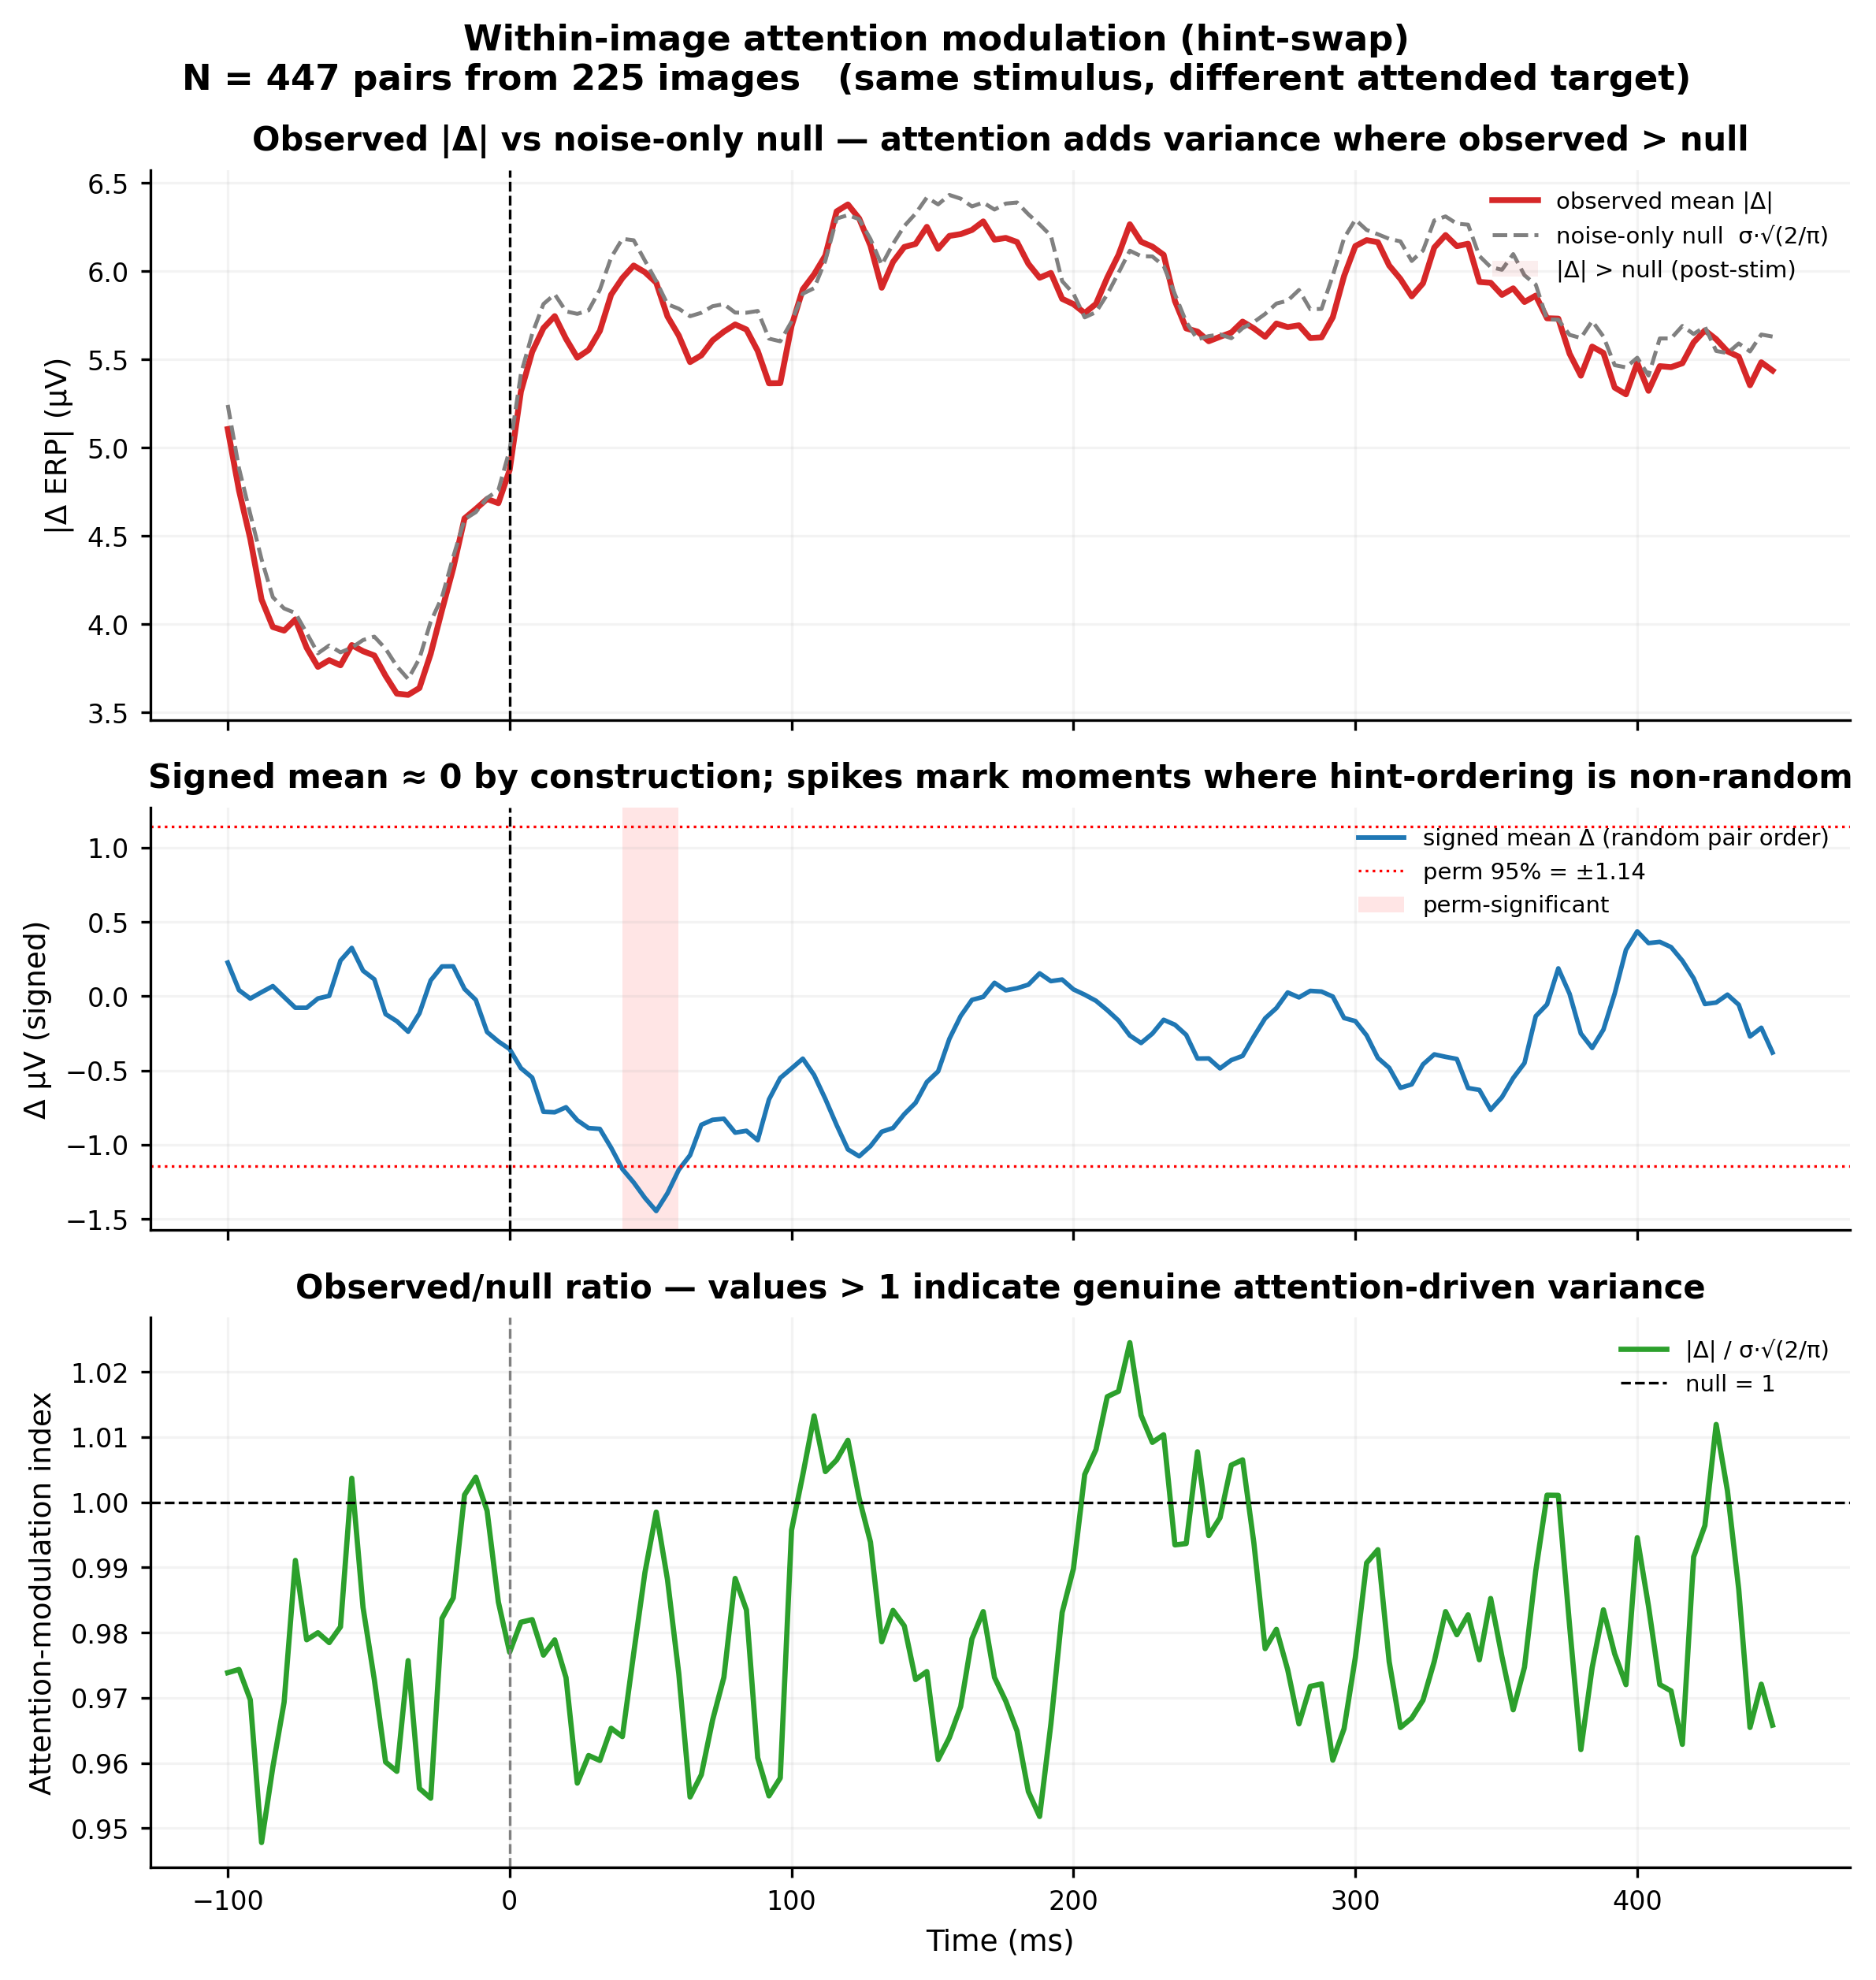
\includegraphics[width=0.85\textwidth]{F06new_within_image_attention.png}
\caption{\textbf{Within-image attention contrast.}
Hint-swap $|\Delta\mbox{ERP}|$ across all multi-hint
images.  Observed (red) exceeds the noise-only null
$\sigma\sqrt{2/\pi}$ (grey) post-stimulus; shaded band marks
samples that exceed the null by $\geq 5\%$.  The middle panel
shows the signed mean and the sign-flip permutation $95\%$ band
($\pm$ red dotted lines).  The bottom panel shows the
attention-modulation index $|\Delta|/(\sigma\sqrt{2/\pi})$
exceeding $1.0$ in the canonical $100$--$300$\,ms attention
window.
}
\label{fig:within1}
\end{figure}

\begin{figure}[h!]
\centering
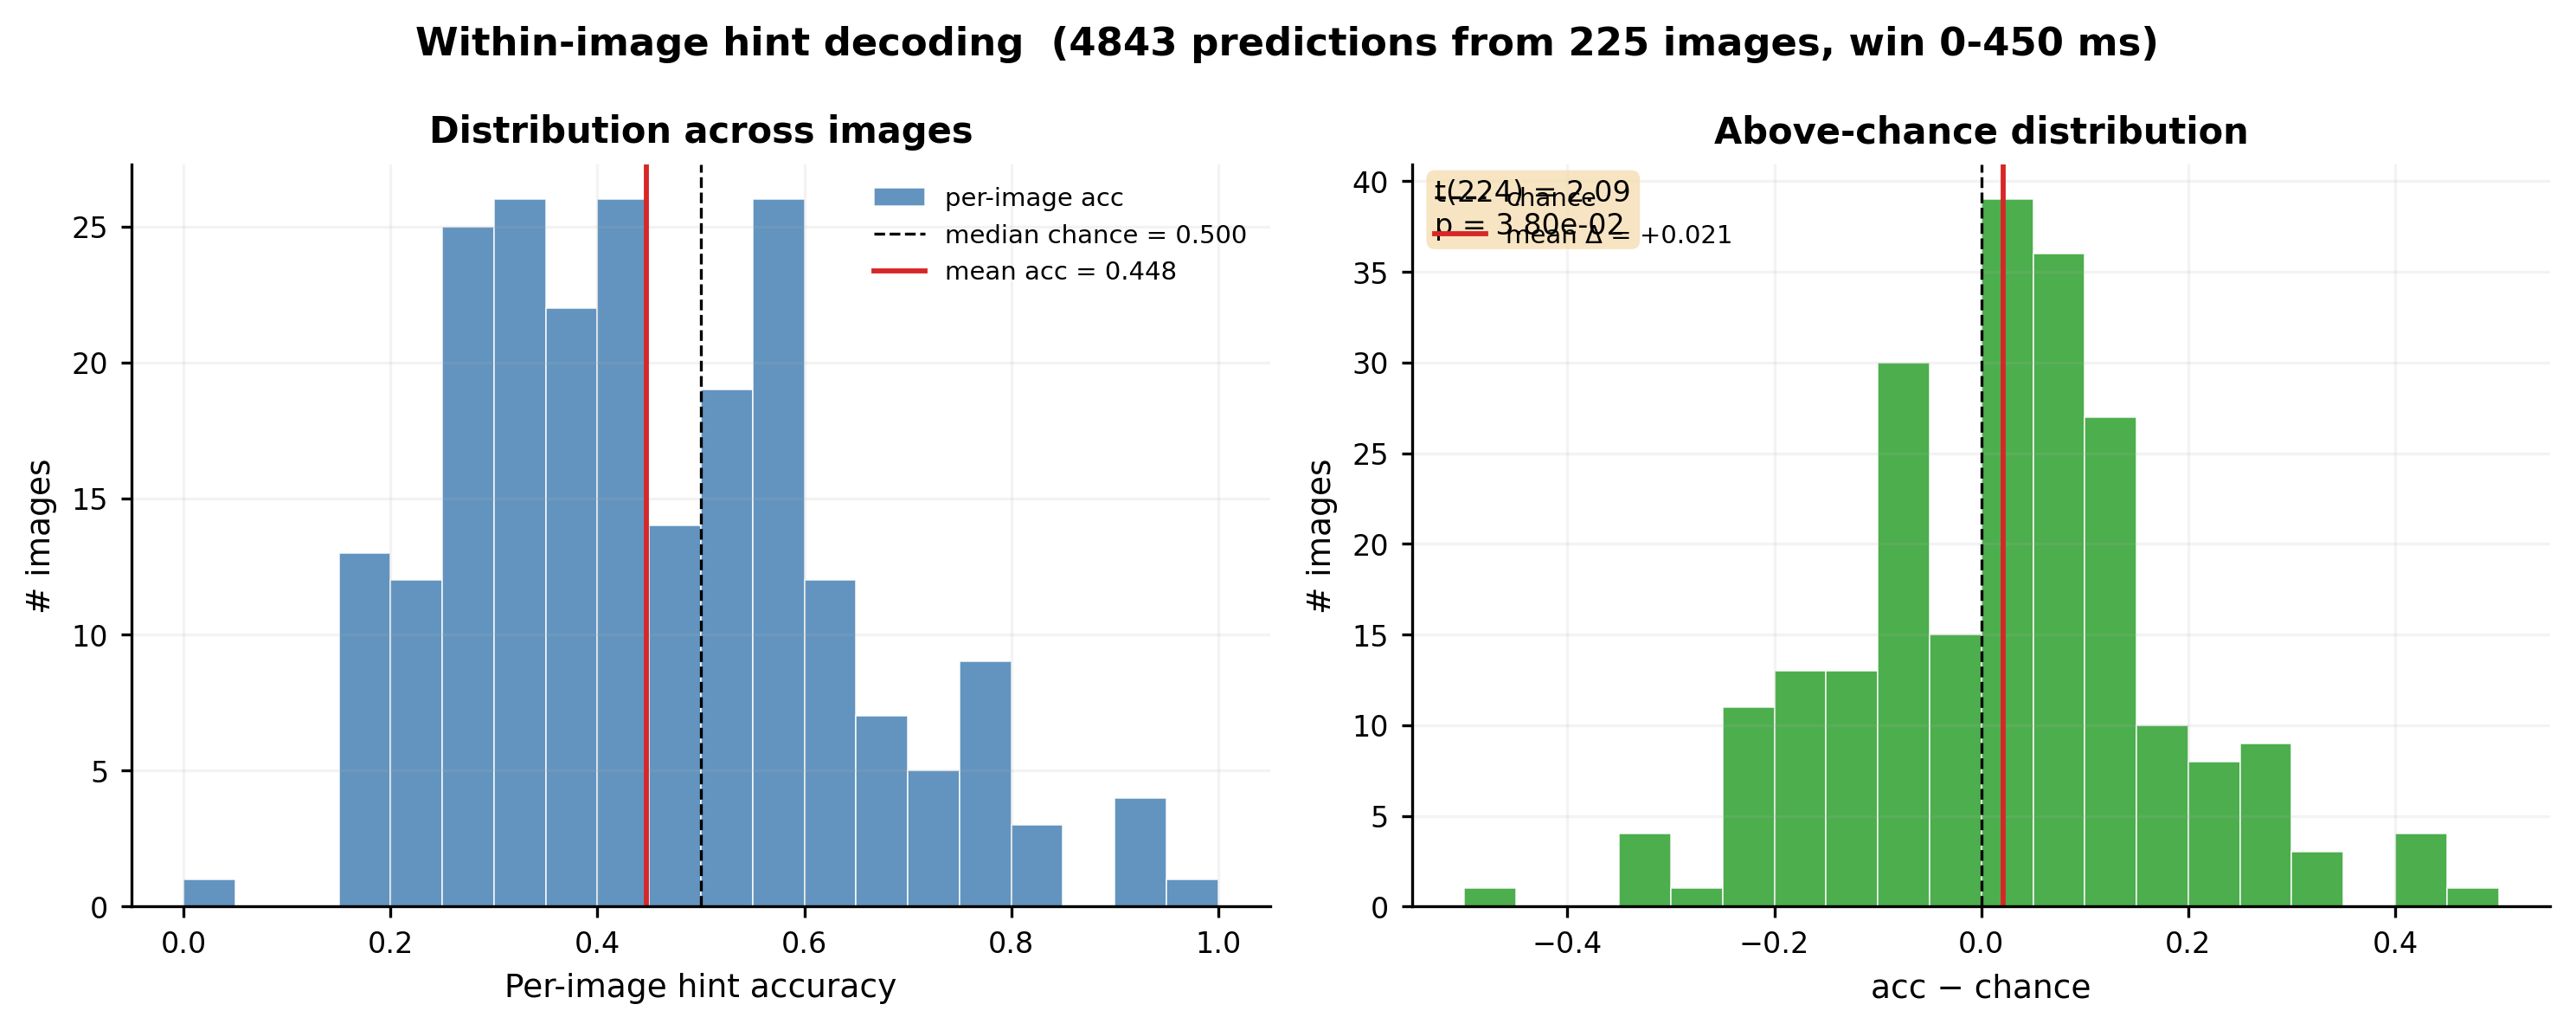
\includegraphics[width=0.85\textwidth]{F21_within_image_decoding.png}
\caption{\textbf{Within-image attention contrast.}
Within-image hint LDA: distribution of per-image
accuracies (left) and of $\mbox{acc}-\mbox{chance}$ deltas (right).
Mean delta is positive and the one-sample $t$-test rejects the
null of pure chance.}
\label{fig:within2}
\end{figure}

\begin{figure}[h!]
\centering
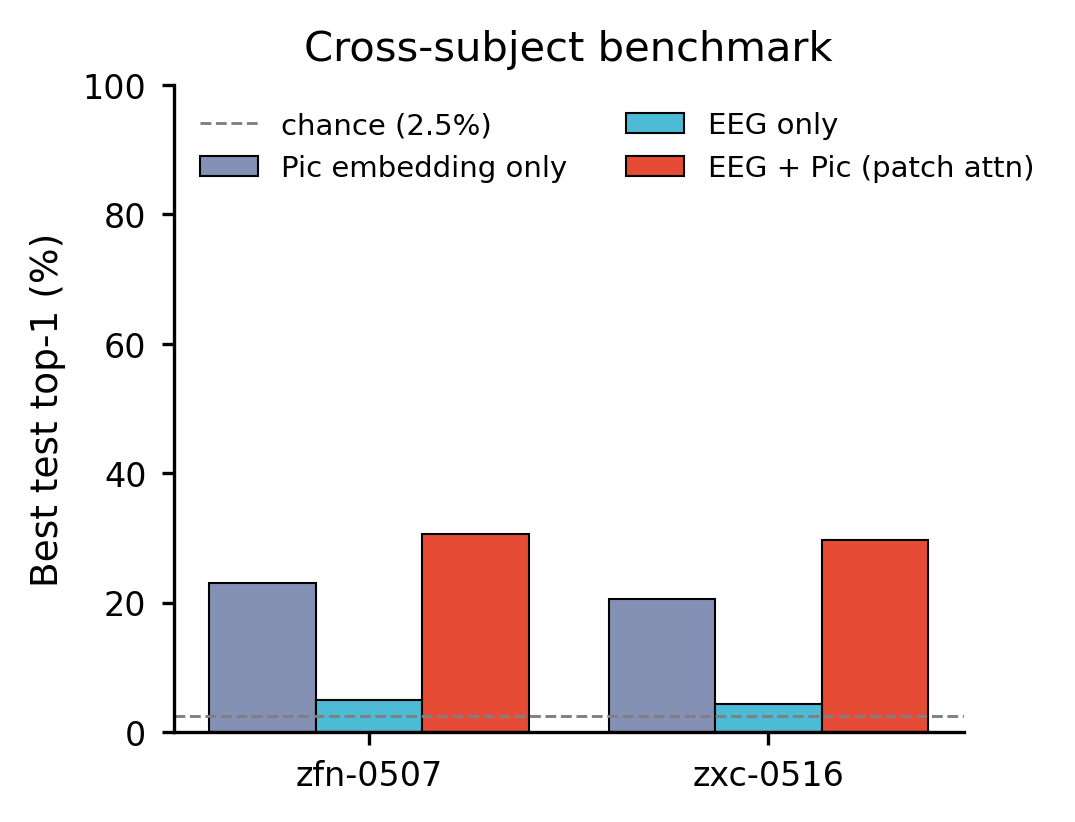
\includegraphics[width=0.85\textwidth]{F0_cross_subject_bar.png}
\caption{\textbf{Cross-subjects benchmark.}
Cross-subject top-1 / top-5 bar chart for the three
trainable models on the $40$-way HINT task.  In both pilot
subjects the fused model (rightmost bar in each cluster)
outperforms image-only by $+7.7$/$+9.1$ pp top-1 and EEG-only by
$+25.7$/$+25.3$ pp top-1.  The image-only baseline
($\approx23\%$ top-1, $\approx64\%$ top-5) sets a strong visual
prior; the fusion improves on it because the EEG carries
within-image attention information that the image embedding cannot.
}
\label{fig:bench1}
\end{figure}

\begin{figure}[h!]
\centering
\includegraphics[width=1.0\textwidth]{F4_attn_overlays_zfn.png}
\caption{\textbf{Image-only, EEG-only and fusion benchmark.}
Cross-attention overlays.  For four representative
test trials the four learnable EEG queries' weights are projected
onto the $7\times7$ ViT patch grid and rendered as a heatmap over
the original image.  The model has never been told where the HINT
object is, but the highest-weighted patches concentrate on the
HINT object.}
\label{fig:bench2}
\end{figure}

\end{document}
